\documentclass[11pt,conference]{IEEEtran}
\IEEEoverridecommandlockouts
\usepackage{cite}
\usepackage{amsmath,amssymb,amsfonts}
\usepackage{algorithmic}
\usepackage{graphicx}
\usepackage{textcomp}
\usepackage{xcolor}
\def\BibTeX{{\rm B\kern-.05em{\sc i\kern-.025em b}\kern-.08em
    T\kern-.1667em\lower.7ex\hbox{E}\kern-.125emX}}
\begin{document}

\title{Automated Essay Scoring \\Using Neural Networks}

\author{\IEEEauthorblockN{Yanchen Wang}
\IEEEauthorblockA{\textit{Analytics Department} \\
\textit{Georgetown University}\\
yw516@georgetown.edu}
\and
\IEEEauthorblockN{Xintong Zhao}
\IEEEauthorblockA{\textit{Analytics Department} \\
\textit{Georgetown University}\\
xz377@georgetown.edu}
\and
\IEEEauthorblockN{Zhen Zhong}
\IEEEauthorblockA{\textit{Analytics Department} \\
\textit{Georgetown University}\\
zz197@georgetown.edu}
}

\maketitle

\begin{abstract}
Automated Essay Scoring (AES) is an effective way to reduce cost and it provides more consistent grading results than human grader. However, designing an auto-scoring method that is close enough to human grader requires a solid background in mathematics and statistics. 
In this project, we introduce two auto-scoring models. One model applies natural language processing (NLP) method to select features and uses neural network to predict the essay score. The other model uses each essay as an input and uses recurrent and convolutional neural network to predict scores. 
\end{abstract}

\begin{IEEEkeywords}
automated essay scoring, recurrent neural network, convolutional neural network, LDA
\end{IEEEkeywords}

\section{Introduction}
The Automated Essay Scoring (AES) integrates the knowledge of Natural Language Processing and Statistical Analysis and automatically returns a score for the input text.

To achieve a similar performance to human grader, one major challenge is feature selection. Good features tend to increase the performance of the model. To select features, In the first model, we apply Latent Dirichlet Allocation (LDA) topic modeling, N-gram analysis to extract the main content of input text, then we feed our features to both recurrent and artificial neural network. In the second model, we use essays as input and use neural networks to automatically select features from essays and predict scores.  

\section{Related Work}

Automated essay scoring (AES) has a long history. Educational Testing Service (ETS) offered e-rater starting in 1999 [1]. In 2012, the Hewlett Foundation sponsored a competition on Kaggle called the Automated Student Assessment Prize [2]. During the competition, there were many models invented to accurately grade essays. Many models use hand-crafted features in their machine learning model. However, those hand-crafted features promotes teaching to test that students learn to write essays to meet features in AES instead of learning to write good essays. In our model, we use two approaches. First, we use essay responses as direct inputs and use recurrent and convolutional neural network to automatically learn features from essays to predict scores of essays. Second, we create some features from essays such as length, number of unique words and relative between essay and its prompt. Then, we feed those predictors into neural network to predict scores of essays.

\section{Datasets}

The dataset was obtained from Kaggle. There are six essay sets and each set has a prompt. There are two types of prompts: argumentative/persuasive, which usually has one sentence statement and asks writers to write their opinions about the statement. The other type of prompt is source dependent responses that writers first read an extract from a book or article then writer respond to a question from the text. All essays  were written by students ranging in grade levels from Grade 7 to Grade 10 and range from an average length of 150 to 550 words per response.During data processing, we first tokenize each essay and remove all stop words such as "a", "I", etc..
\begin{table*}[htbp]
\caption{Dataset Description}
\begin{center}
\begin{tabular}{|c|c|c|c|c|}
\hline

\textbf{Essay Set} & \textbf{Type}& \textbf{Score Range}& \textbf{Average Length}& \textbf{Number of Essays} \\
\hline
1& Argumentative/Persuasive & 2 - 12&  350 Words & 1,785\\
\hline
2& Argumentative/Persuasive & 2 - 12&  350 Words & 1,800\\
\hline
3 & Source Dependent Responses & 0 - 6&  150 Words & 1,726\\
\hline
4 & Source Dependent Responses & 0 - 6&  150 Words & 1,772\\
\hline
5 & Source Dependent Responses & 0 - 8&  150 Words & 1,805\\
\hline
6 & Source Dependent Responses & 0 - 8&  150 Words & 1,800\\
\hline
\end{tabular}
\label{tab1}
\end{center}
\end{table*}

\section{Methods}

We develop two models using neural network. The first model uses recurrent neural network and convolutional neural network using the whole essay to predict its score. The second model selects features from each model and use those features as predictors to predict its score using artificial neural network and recurrent neural network. 

\subsection{Recurrent and Convolutional Neural Network}\label{AA}
Figure 1 shows the architecture of the neural network.
\begin{itemize} 
\item \textbf{Word embedding}: each word in the essay (after removing all stop words) would be projected into 64 dimensional space. 
\item \textbf{Neural Network Fitting}: Three different models are used in this step. First, only deep recurrent neural network (RNN) is used. We create three layers and in each layer. In each recurrent layer, we choose long short-term memory (LSTM) units. Second, only convolutional neural network (CNN) is used. We use three layers of one dimensional convolutional neural network with max pooling. Last, we use both CNN and RNN that we create one 1 dimensional convolutional layer with max pooling and one recurrent layer to train the dataset.  
\item \textbf{Output}: If cross entropy loss function is used, the goal is to predict exact score (classification problem) and the final output would be discrete values for predicted score. If mean squared error loss function is used, the goal is to minimize error between scores from human grader and scores from the model. The output would be numeric values (in decimals). In order to get a score for the essay, we round each numeric score into discrete, whole value score.
\end{itemize}

\begin{figure*}[htbp]
\centerline{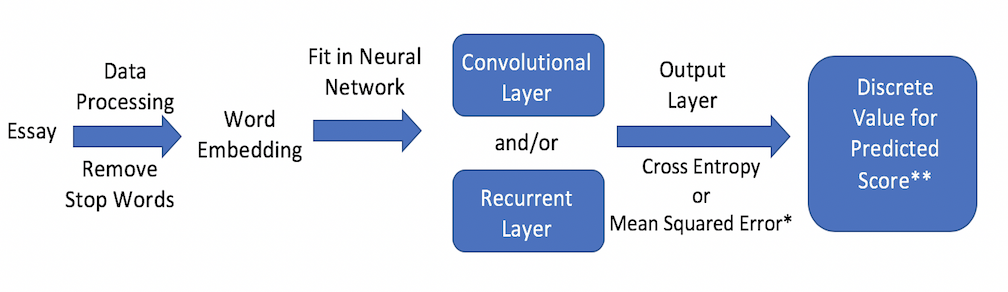
\includegraphics{fig1.png}}
\caption{Neural Network Architecture}
\footnotesize{* If the goal is to predict exact score of the essay, cross entropy loss function would be used. If the goal is to minimize error between real score and predicted score, mean squared error loss function would be used.}\\
\footnotesize{** If mean squared error loss function is used in output layer, the output would be numeric. The numeric value results would be rounded to get predicted score for the essay.}
\label{fig}
\end{figure*}

\subsection{Feature Selection}

In this section, we tried to extract features from each essay and use them to predict score of the essay. 

The key point of feature selection in our case is how to accurately extract the main content and writing pattern of input text data. After removing stop words and stemming process, we firstly apply Latent Dirichlet Allocation (LDA) method to extract the keywords related to the prompt, then use unigram, bigram and trigram analysis to search potential writing patterns that could exist in given document, and compute their frequencies. 

Other than N-gram analysis and LDA topic modeling, we also select length of the essay, number of sentences, average sentence length, word length, unique word length and number of unique words, all predictors include values before and after removing stop words. Most importantly, we create a feature that measures the ``relativeness'' to the prompt, shown as ``number of synonyms/antonyms''.

For the main content of the essay prompt, we use corpus from NLTK [3] to find all words that are related to the main content. Then, while processing the input text, we check if each word is related to the essay prompt and count the frequency of synonyms and antonyms. 

After generating all features above, we implement artificial neural network and recurrent neural network using all features extracted from each essay. We created a vector in 71 dimensional space that contains all features from each essay.

We build a regression model using artificial and recurrent neural network with mean squared error as loss function. Outputs from the two neural networks are continuous numeric values and we round the result into integers and use them as score for each essay. 

\subsection{Regularization and Tuning}

In all neural networks we build, we use early stopping as our regularization method. 
Figure 2 shows loss values in training and validation set. Early stopping helps us prevent overfitting in neural networks. In Tuning process, we choose different learning rates and picked the optimal one. 

\begin{figure}[htbp]
\centerline{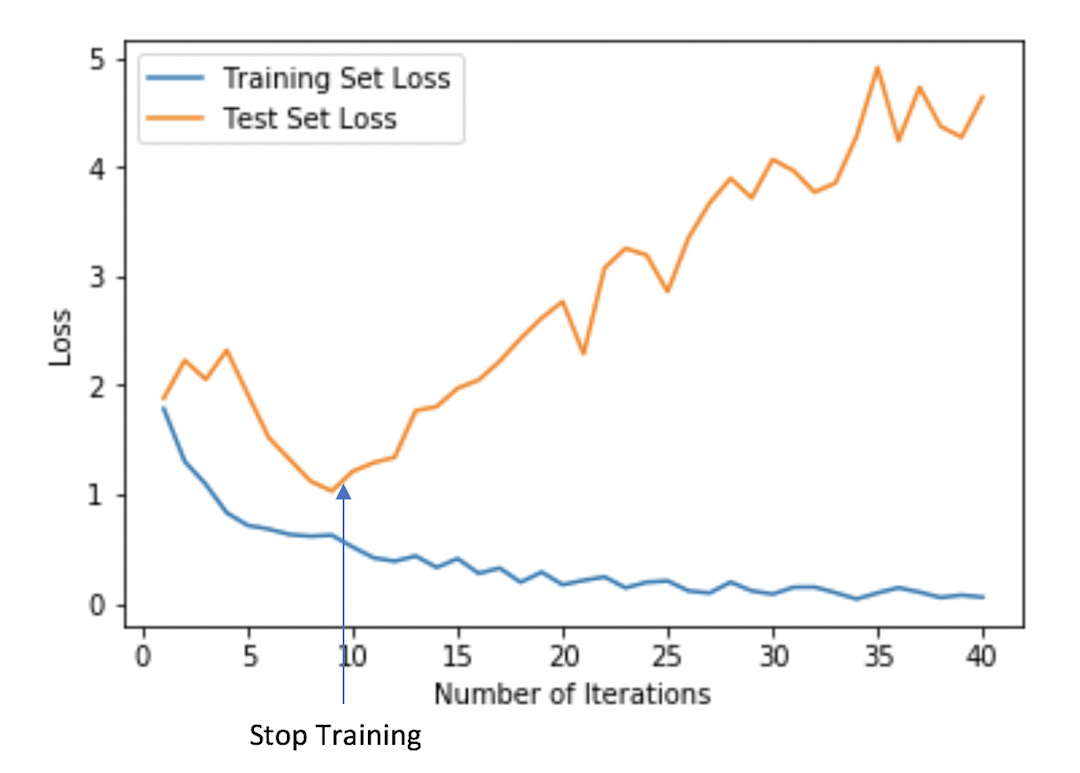
\includegraphics{fig2.png}}
\caption{Early Stopping}
\label{fig}
\end{figure}


\section{Results}

In all networks we build, we split the dataset into training and validation set. In this section, all results are results from validation set. In addition to exact accuracy, we also tried to use $\pm$ 1 point accuracy, which measures accuracy if our predicted score is within $\pm$ 1 point from the real score. The reason we introduce this measurement is that there are uncertainties for human graders. For example, it is very likely that one grader gives a score 7 and the other grader gives a score 8 on the same essay. Hence, we will introduce such uncertainties into out models. Table 2 shows results from recurrent and convolutional neural network using each essay as direct input. 

\begin{table*}[htbp]
\caption{Results from Recurrent and Convolutional neural network}
\begin{center}
\begin{tabular}{|c|c|c|c|c|c|c|c|c|c|c|c|c|}
\hline

\textbf{Model} &\multicolumn{6}{|c|}{\textbf{Essay Set/Exact Accuracy}} &\multicolumn{6}{|c|}{\textbf{Essay Set/$\pm$ 1 point Accuracy}} \\
\cline{2-7} 
\cline{8-13} 
\textbf{Type}&1 &2&3&4&5&6&1 &2&3&4&5&6\\
\hline
RNN& 0.63&0.59&0.58&0.56&0.49&0.49&0.91&0.93&0.88&0.85&0.86&0.88\\
\hline
CNN&0.52&0.51&0.52&0.54&0.52&0.47&0.87&0.86&0.87&0.83&0.84&0.84\\ 
\hline
RNN + CNN&0.56&0.54&0.56&0.58&0.51&0.50&0.87&0.87&0.85&0.82&0.85&0.84\\
\hline
\end{tabular}
\label{tab1}
\end{center}
\end{table*}

\begin{table*}[htbp]
\caption{Results from feature selection}
\begin{center}
\begin{tabular}{|c|c|c|c|c|c|c|c|c|c|c|c|c|}
\hline

\textbf{Model} &\multicolumn{6}{|c|}{\textbf{Essay Set/Exact Accuracy}} &\multicolumn{6}{|c|}{\textbf{Essay Set/$\pm$ 1 point Accuracy}} \\
\cline{2-7} 
\cline{8-13} 
\textbf{Type}&1 &2&3&4&5&6&1 &2&3&4&5&6\\
\hline
RNN&0.61&0.57&0.55&0.56&0.53&0.47& 0.93&0.92&0.89&0.88&0.92&0.87\\
\hline
ANN&0.56&0.55&0.57&0.51&0.56&0.48&0.92&0.89&0.88&0.86&0.88&0.86\\
\hline
\end{tabular}
\label{tab1}
\end{center}
\end{table*}

\section{Discussion of Results}

Since the dataset is from a Kaggle competition in 2010, we use results in 2010 as our benchmark. In 2010, the best model used features such as length of essay, average length of sentences, number of unique words and etc. extracted from essays and feed those features in predictive models such as decision tree, regression [2]. Our result, in terms of accuracy, is a little bit better than results in Kaggle especially performance one essay set 1 and 2. For neural networks using essay as an input, we also tried simpler methods such as softmax as benchmark. Our results using RNN and CNN are similar to results from softmax.

The main difference between our model and models developed in 2010 is the use of RNN, CNN and NLP. In the first model, we use the essay as an input and let neural networks automatically learn features from all essays and predict a grade. In traditional models, they used hand crafted features that writers can follow a particular format to get a high grade. However, our models are ``black box'' models that it is almost impossible for writer to follow a particular format to get a high score. Moreover, performance of our model would become better as dataset gets larger and more robust. 

Our model has the best performance in essay set 1 and 2. Those essays have the same type, argumentative/persuasive. We think this happens because writing style in argumentative/persuasive essays differ a lot from each other that RNN and CNN using essays as direct inputs could learn from the diversity among essays and have better prediction results. 

We think that our models are limited by the size of the dataset. In each essay set, there are about 1,800 essays. Performance of our model would be better if we could get a larger dataset, at least 18,000 essays in each essay set. 

\section{Conclusions}

In this paper, we present neural networks and NLP models for automated essay grading using RNN, CNN and features extracted from essays. Performance of our models are not significantly better than existing models. We think there are potentials to improve our model. In the future, we could collect more essays to train our model, try different word embedding methods and use other NLP tools to extract other features from essays. 

\begin{thebibliography}{00}
\bibitem{b1} Burstein ``The E-rater(R) Scoring Engine: Automated Essay Scoring with Natural Language Processing'', in: Automated Essay Scoring: A Cross-Disciplinary Perspective. Shermis, Mark D., and Jill Burstein, eds. Lawrence Erlbaum Associates 2003, p. 113.
\bibitem{b2} Kaggle, ``The Hewlett Foundation: Automated Essay Scoring.'' RSNA Pneumonia Detection Challenge  2010.
\bibitem{b3} Bird, Steven, Edward Loper and Ewan Klein (2009), Natural Language Processing with Python. O?Reilly Media Inc.
\end{thebibliography}
\vspace{12pt}

\end{document}
